\chapter{Disclination response and helical dirac hinge states}
\section{BBH model and its corner states}
Benalcazar, Bernevig, and Hughes (BBH) proposed the inaugural model for intrinsic higher-order topological phases\cite{benalcazar2017quantized}. The BBH model, a two-dimensional generalization of the one-dimensional SSH model, showcases corner states that arise from the bulk topology and are protected by crystalline symmetries. This model follows a $\mathbb{Z}_2$ classification with the quadrupole moment serving as its topological invariant. A quadrupole moment of 0 signifies a trivial bulk, void of corner states, while a quadrupole moment of $1/2$ indicates a non-trivial bulk.

 We consider a spinless square lattice with nearest-neighbor hopping which alternates between weak and strong coupling shown in fig \ref{fig:bbh}. The tightbinding Hamiltonian is:
 \begin{equation}
     H=-\sum_{<i,j>}t_{i,j}c^\dagger_ic_j
 \end{equation}
 where $i,j$ are the lattice site and $t_{i,j}$ altenates between $t$ and $t'$. A $\pi$-flux can be introduced to each plaquette which lead to the minus sign in one of the coupling for each plaquette and we end up with a four atom unit cell  shown in fig \ref{fig:bbh}. The system has four fold rotation symmetry and the hopping dimerized along the $x$ and $y$ direction. 

  \begin{figure}[h]
    \centering
    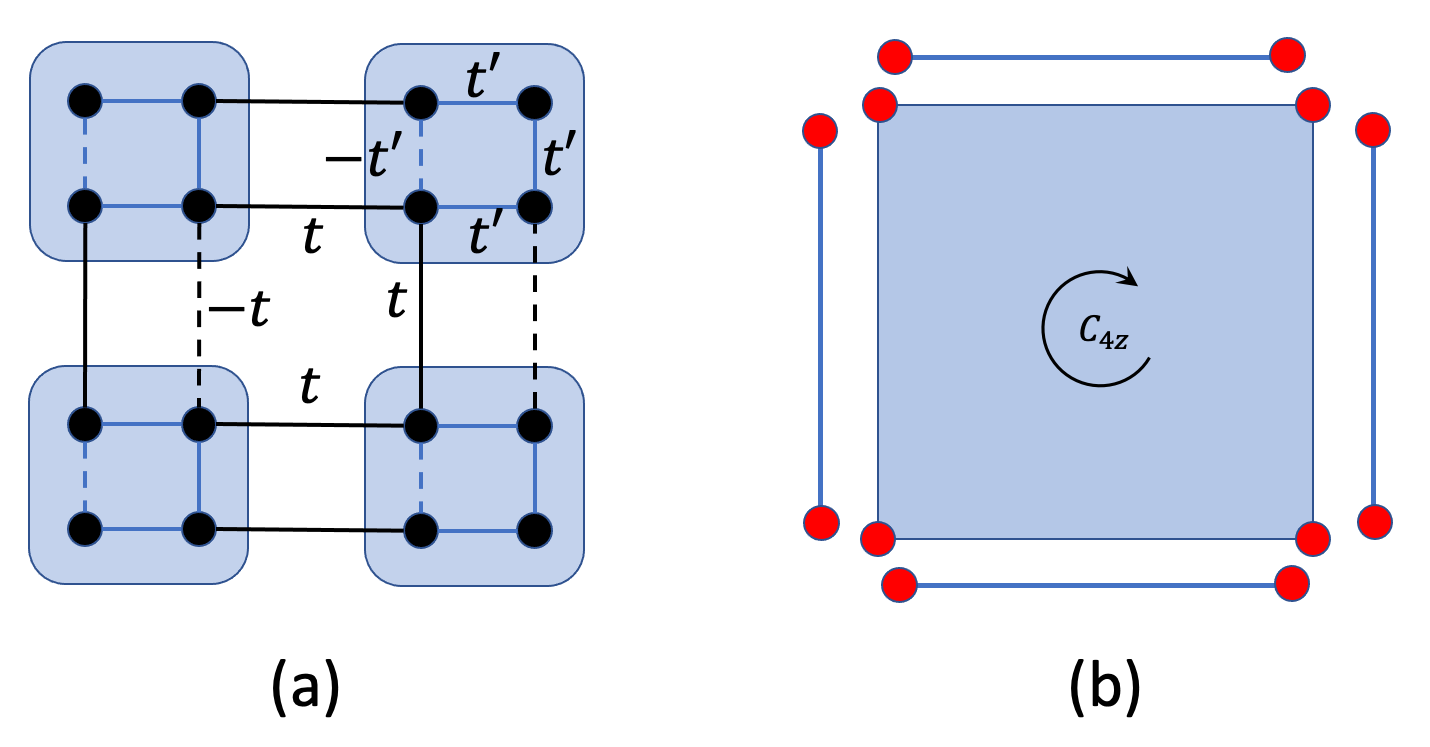
\includegraphics[width =\textwidth]{images/bbh.png}
    \caption{(a)BBH model in a square lattice. The blue square is the unit cell. Dash lines represent the negative sign in the coupling strength. (b) The corner states of BBH model stacked with 1D chain. They are pinned to the corner as long as the stacking chains preserve the four fold rotation symmetry.}
    \label{fig:bbh}
\end{figure}

The model Hamiltonian is
\begin{equation}
\begin{aligned}
    H(k_x,k_y) = &(t'+t\cos{k_x})\tau_x - t\sin{k_x}\tau_y\sigma_z\\
    &- (t'+t\cos{k_y})\tau_y\sigma_y-t\sin{k_y}\tau_y\sigma_x
\end{aligned}
\end{equation}
where $\sigma$ and $\tau$ are the degrees of freedom within the unit cell. The system preserves reflection symmetry on $x$ and $y$ direction and a four-fold rotation along $z$-axis.
\begin{align}
    H(k_x,k_y) = M_xH(-k_x,k_y)M_x^{-1}\\
    H(k_x,k_y) = M_yH(k_x,-k_y)M_y^{-1}\\
    H(k_x,k_t) = C_{4z}H(k_y,-k_x)C_{4z}^{-1}
\end{align}
where $M_x = \tau_x\sigma_z$, $M_y = \tau_y\sigma_x$ and
\begin{equation}
C_{4z}=\begin{pmatrix}
0&\sigma_0\\-i\sigma_y&0
\end{pmatrix}.
\end{equation}
This Hamiltonian can then be smoothly transformed to a Dirac form with mass term using $t'=-t+m/2$:
\begin{equation}
\label{eq:Hbbh}
\begin{aligned}
H\left(k_1, k_2\right)= & \Gamma_0\left[m+t\left(2-\cos k_1-\cos k_2\right)\right] \\
& +\Gamma_1 t \sin k_1+\Gamma_2 t \sin k_2 \\
& -\Gamma_4 t\left(\cos k_1-\cos k_2\right)
\end{aligned}
\end{equation}
where $\Gamma$ are the Dirac matrices and anticommute with each other, $\Gamma_0=-\frac{1}{\sqrt{2}}(\Gamma_++\Gamma_-)$ and $\Gamma_4=-\frac{1}{\sqrt{2}}(\Gamma_+-\Gamma_-)$.

When the mass term $m$ shifts from negative to positive, a gap closing point occurs at $m=0$. This point could represent a phase transition, and it's possible to determine whether this gapless phase transition is topological. If another mass term can be found that anticommutes with all the $\gamma$ matrices while preserving symmetries, then a smooth transformation from the $-m$ phase to the $+m$ phase is possible without closing the gap, by passing through another mass term. In this case, the two phases are topologically identical. However, if no other mass term can be found that satisfies the symmetry constraints, the phase transition point is deemed topological.

For Hamiltonian \ref{eq:Hbbh}, it is impossible to find any mass term that preserves symmetries. As a result, the gap closing point at $\mathbf{k}=(0,0)$ and $\mathbf{k} = (\pi, \pi)$ when $m=0$ represents a topological phases transition. $m=0$ represent the inter-cell and intra-cell coupling strength equals to each other $|t/t'|=1$. However if we relax the requirement for four-fold rotation symmetry, a mass term $M=\Gamma_4$ can be introduced and the bulk topology is always trivial. Hence the topological phase in the BBH model is protected by the $C_{4z}$ symmetry. 

In the presence of $C_{4z}$ symmetry, the BBH model hosts topological phases when $|t/t'|<1$ or $-4t<m<0$. A topological invariant can be defined as the quantized quadrupole moment:
\begin{equation}
    q_{xy} = 2ep_xp_y
\end{equation}
where $p_x$ and $p_y$ are the polarizations calculated through the nested Wilson loops as a bulk property.
\begin{equation}
    p_{x/y} = \begin{cases}
        0, \quad\quad \text{for} |t/t'|>1\\
        1/2,\quad\text{for} |t/t'|<1
    \end{cases}
\end{equation}
The most comprehensive classification based on polarizations would be $\mathbb{Z}_2\otimes\mathbb{Z}_2$, however, the $C_{4z}$ symmetry further reduces the classification of the BBH model to $\mathbb{Z}2$. The topological phase is associated with a quantized quadrupole moment of $e/2$, corresponding to corner charges or corner states (in superconducting systems) as the boundary signature, whereas $q{xy}=0$ designates the trivial state. These corner states or charges are derived from the bulk invariant, indicating their intrinsic nature. As long as the lattice termination modification is compatible with the $C_{4z}$ symmetry, the gapless states are pinned to the corners. One approach to modify the boundary termination involves stacking one-dimensional chains, characterized by gapless ends, along the boundary as illustrated in Figure \ref{fig:bbh}(b). Due to the $C_{4z}$ symmetry, the number of gapless states added to each corner is always even, ensuring that the corner states are never vanished.

\section{Topological defects * move to later}
* defects influence the classification
* physcis phenomena
* disclination details
\section{Topological Disclination}
% \lipsum[1-20]









\section{DISCLINATION RESPONSE}
We consider both the (even) vertex-type and the (odd) plaquette-type disclination illustrated in Figure \ref{fig:disclination}. The even and odd disclinations are related to each other by plaquette-vortex duality, which is described by half unit cell translation along the $xy$ direction in our model. 

In even disclination, hopping term with gapping $\delta H_{xy}^{topo}$ possesses uncoupled helical mode at the center of disclination with Frank angle $\Omega = \pi/2$ and the half unit cell translated gapping mass term will not possess any helical mode at the center of the disclination. However, the existence of the helical mode at disclination is origin dependent. In odd disclination instead, the half unit cell translated gapping term will possess uncoupled helical modes at the center of disclination while the original gapping term will not leave behind uncoupled helical mode at the center of disclination. {\color{red}(Draw a diagram with 4 cases: (1) $\delta H$ leaving uncoupled hinge node/mode at the center of even (2) $\delta H$ leaving no uncoupled hinge node at the center of odd (3) Half translated $\delta H$ leaving no uncoupled hinge node at the center of even (4) Half translated $\delta H$ leaving uncoupled hinge node at the center of odd.)}

%which in our model is described by the $T_x$ or $T_y$ translations that interchanges the inter-cell and intra-cell hopping terms.

\begin{figure}[htbp]
    \centering\includegraphics[width=0.5\textwidth]{hingestate.png}
    \caption{(Left) Type-1 disclination centered at a triangular plaquette with an odd number of translations around its boundary, $\mathbf{T} = 1 \mod 2$. (Right) Type-0 disclination centered at a trivalent vertex with an even number of translations around its boundary, $\mathbf{T} = 0 \mod 2$.} \label{fig:disclination}
\end{figure}

%For the even disclination with broken $T_x$ and $T_y$ symmetry (diagram), there are three dangling helical modes that are not gapped out completely by the gapping terms breaking $T_x$ and $T_y$ symmetries ($\delta H_z$ in Eqn (\ref{z_gapping_nontrivial}) and $\delta H_{xy}^{trivial} = \delta H_{xy, +} + T_x \delta H_{xy, -} T_x^{-1}$). For these cases, we can see that the existence of hinge states from the XY-plane slice of the model ({\color{red}diagram}). We could also consider the dual (odd) description of the even disclination with broken $T_x$ and $T_y$ symmetry by interchanging the strong (solid line) and weak (dotted lines) bonds and deduce the existence of the 3 hinge helical modes at the center of the plaquette ({\color{red}diagram}).  

%The absence of the hinge helical modes in gapping terms respecting $T_x$ and $T_y$ translations can be similarly deduced from ({\color{red} diagram}). For both the even and odd disclinations with $T_x$ and $T_y$ translational symmetry, there are no helical modes left uncoupled by the strong (solid line) bonds, thereby forbidding the existence of hinge states in the disclinations considered. $\delta H_{trivial}$ in Eqn (\ref{trivial_gapping}) is an example of a gapping term that respects $T_x$ and $T_y$ without any hinge modes.

Armed with our results on the $z_8$ symmetry indicator and weak indices, we employ K-theoretic technique to conjecture a form of $\mathbb{Z}_2$ disclination index theorem that predicts the existence of helical mode. We denote the equivalence class of the Hamiltonian $\delta H_{xy}^{topo}$ as $[ H_1 ]$ and the half-translated $(T_{1/2}^{r})^{-1} \delta H_{xy} T_{1/2}^r$ as $[ H_2 ]$. We summarized these results in table \ref{sub-K-group}. $\mathbf{T}$ is to be understood as the evenness/oddness of translation surrounding the disclination and $\mathbf{G_{\nu}} = \nu (\mathbf{G_1} + \mathbf{G_2})$. The sub-K-group for the classification in table \ref{sub-K-group} is given by
\begin{equation}
    K' = \langle H_1, H_2, H_1 \oplus H_2, 1 \rangle = \mathbb{Z}_2 \oplus \mathbb{Z}_2 .
\end{equation}

With these results, we conjecture the following $\mathbb{Z}_2$ disclination index theorem indicating the presence of helical mode at the center of disclination
\begin{equation}
    \Theta = \left[ \mathbf{G_{\nu}} \cdot \mathbf{T} + \frac{\Omega}{2 \pi} z_8 \right] \mod 2 ,
\end{equation}
where the Frank angle $\Omega = \pi / 2$ at disclinations. Note that this form of index theorem is reminiscent of the index theorem proposed in \cite{Teo_2013, Teo_disclination_2014} as these work discussed topological superconductor with $C_4$ and inversion symmetry. 

\begin{table}[h]
\begin{tabular}{c|cccc}
$K'$  & $[ H_1 ]$ & $[ H_2 ]$ & $[ H_1 ] \oplus [ H_2 ]$ & $[ 1 ]$  \\
\hline 
$z_8$ indicator &  4 & 0 & 4 & 0 \\
Weak indices $\{ \nu_1 \nu_2 \nu_3 \}$ & (110) & (110) & (000) & (000) \\
$\mathbf{G_{\nu}} = \nu (\mathbf{G_1} + \mathbf{G_2})$ & 1 & 1 & 0 & 0 \\
Type-0 (even, $\mathbf{T} = 0 \mod 2$) & Yes & No & Yes & No \\
Type-1 (odd, $\mathbf{T} = 1 \mod 2$)& No & Yes & Yes & No \\
\end{tabular}
\caption{The sub-K-group table showing the existence of helical mode at the center of disclination (indicated by Yes/No in the last 2 rows). $\mathbf{G}$ and $\mathbf{T}$ values here are to be understood as $\mathbf{G} \dots \mathbf{T}$, $[ H_1 ] \oplus [ H_2 ]$ is taken from the adding $[ H_2 ]$ bands to $[ H_1 ]$ in K-theoretic sense and $[ 1 ]$ is the equivalence class of trivial insulator.} \label{sub-K-group}
\end{table}

%\subsection{Vortices}

{\color{red}(Show that the z8 index is origin dependent with a nontrivial weak index, and that the $(0,0)$ and $(\pi , \pi)$ CDW phases have $\{ 4|01 \}$ and $\{ 0|01 \}$, and that the strong sector corresponds to an origin (half-translation)-dependent 90 degree disclination response (such that the difference between the $(0,0)$ and $(\pi , \pi)$ phases is a TCI with an origin-independent nontrivial disclination response)}

%We can project eq(13) to $C_2$ symmetric subspace
%\begin{equation}
%    H^\pm=\mp2\tau_x\mu_zs_z(u_1-\tilde{u}_1)k_rk_s+\tau_z\mu_zu_2(k_r^2-k_s^2)+2v_0\tau_yk_z
%\end{equation}
%where $H^\pm$ have the rotation eigenvalue $\pm i$.
%Each sector has an artificial symmetry $S=\sigma_z\tau_z$, the %Hamiltonian $H^+$ can be furthur block diagonlized to two %sectors
%\begin{equation}
%    H^+_\pm=\pm\tau_x(u_1-\tilde{u}_1)k_rk_s+\tau_z\mu_zu_2(k_r^2-k_s^2)-2k_zv_0\tau_y\mp (m_1\tau_z\mu_y+m_2\tau_z\mu_x)
%\end{equation}

\section{Misc}
\subsection{Symmetry Breaking to Point Group 4}

{\color{red}(Break the symmetry down to point group 4 (or 422 if you had Mx,My, better matches TaSeI) and show that the same arguments still apply without modification, but are no longer symmetry-indicated (the z8 is just the rotation anomaly index from \cite{TCISurfaceRotationAnomaly}, so it only requires C4z and T, no inversion)

(This will include either a Wilson loop or other creative winding index for the origin-dependent z8 (or z8 mod 4, at least)

(relax C4, show that there still exist situations where z-directed helical modes remain)}

